%------------------------------------------------------------
\title[11 - 递归 II]
{11 - 递归 II}

\subtitle{C++ 程序设计进阶}

\author[Beiyu Li]
{Beiyu Li\\
\texttt{<sysulby@gmail.com>}}

% \institute[SOJ]
% {Sicily Online Judge}

\date[\today]
{\number\year 年 \number\month 月 \number\day 日}
%------------------------------------------------------------


\begin{document}

\author[sysulby]
{SOJ 信息学竞赛教练组}

\begin{frame}
    \titlepage
\end{frame}
\setcounter{framenumber}{0} % 标题页不编号


\section{复习回顾}

%------------------------------------------------------------
\begin{frame}[fragile]
    \frametitle{递归分析问题的重点}

    \begin{itemize}
        \item 将原问题分解为一个或多个性质相同、规模更小的子问题
        \begin{itemize}
            \item 子问题与原问题性质相同,调用函数自身解决(自我调用)
        \end{itemize}
        \item 解决子问题后,经过组合/操作形成原问题的答案
        \item 最简子问题直接解答,无需分解(结束条件)
    \end{itemize}
    
\end{frame}
%------------------------------------------------------------

%------------------------------------------------------------
\begin{frame}[fragile]
    \frametitle{例 11.1:数的精致度}

    \only<1>{
        \begin{exampleblock}{编程题}
            \begin{itemize}
                \item 一个正整数 $n$ 的“精致度”,为该数的所有真因子的“精致度” 
                    之和。特别地,$1$ 的“精致度”为 $1$ 。\\
                    \vspace{1em}
                    输入一个正整数 $n (1 \le n \le 10^6)$ ,输出 $n$ 的“精致度”。
                \item 输入样例 \\
                    \lstinline|4|
                \item 输出样例 \\
                    \lstinline|2|
            \end{itemize}
        \end{exampleblock}
    }

    \only<2-8>{
        \begin{itemize}
            \item 真因子:一个正整数 $n$ 的真因子为 $1 \sim n-1$ 范围内 $n$ 的因子
                
            \item<3-> 样例解释
            \begin{columns}
                \column{.03\textwidth}
                \column{.50\textwidth}
                \begin{itemize}
                    \item $4$ 的真因子有: $1, 2$
                    \item<4-> $1$ 的精致度 $= 1$
                    \item<5-> $2$ 的真因子有: $1$,因此,\\ $2$ 的精致度 $= 1$ 的精致度
    
                \end{itemize}

                \column{.47\textwidth}
                \begin{tikzpicture}[node distance=0.5cm and -0.8cm, % 控制节点之间的距离
                    every node/.style={rectangle, draw, rounded corners, align=center, minimum width=1cm, minimum height=0.5cm}  % 设置节点样式
                ]
        
                % 定义节点
                \node (n1) [draw=none] {$4$ 的精致度};
                \uncover<7->{\node (n0) [below=of n1, draw=none] {$+$};}
                \node (n2) [below left=of n1, draw=none] {$1$ 的精致度};
                \node (n3) [below right=of n1, draw=none] {$2$ 的精致度};
                \uncover<4->{\node (n4) [below=0.02cm of n2, color=red, draw=none] {$1$};}
                \uncover<5->{\node (n5) [below=of n3, draw=none] {$1$ 的精致度};}
                \uncover<6->{\node (n6) [below=0.02cm of n5, color=red, draw=none] {$1$};}
        
                % 绘制连线
                \draw[->] (n1.south) -- (n2.north);
                \draw[->] (n1.south) -- (n3.north);
                \uncover<5->{\draw[->] (n3.south) -- (n5.north);}
        
                \end{tikzpicture}
            \end{columns}

            \uncover<7-8> {
                \begin{flalign*}
                    4 \text{ 的精致度} &= 1 \text{ 的精致度} + 2 \text{ 的精致度} \nonumber \\
                            \uncover<8>{&= \textcolor{red}{2} \nonumber}
                \end{flalign*}
            }

        \end{itemize}
    }

    \only<9-13> {
        \begin{itemize}
            \item 原问题:计算一个数 $n$ 的“精致度”
            \item 子问题:计算 $n$ 的真因子的“精致度”
            \item<10-> \lstinline|calc(x)| 用于计算整数 $x$ 的“精致度”
                \begin{itemize}
                    \item<11-> 原问题和子问题的关系:\\原问题的答案 为 所有子问题的答案之和
                    \item<12-> 枚举 $x$ 的所有真因子,将每个真因子的“精致度”加起来
                        \begin{itemize}
                            \item 递归调用 \textcolor{red}{\lstinline|calc(真因子)|} 计算真因子的精致度
                        \end{itemize}
                    \item<13> 最简子问题:$1$ 的精致度是 $1$
                \end{itemize}
        \end{itemize}
    }

    \only<14> {
        \lstinputlisting[basicstyle=\ttfamily\footnotesize,language=C++,name=calc_x]{ch23/calc_x.cc}
    }

\end{frame}
%------------------------------------------------------------


\section{递归的其他分析方式}

%------------------------------------------------------------
\begin{frame}[fragile]
    \frametitle{递归分析问题}

    \begin{itemize}
        \item 递归的特点是在函数中调用自身,函数是一组实现某个功能的语句,因此递归本质上是在重复执行函数中的语句
        \item 递归分析问题的一种方式:
            \begin{itemize}
                \item 根据解决问题时需要重复执行的操作或功能,明确子问题是什么,给递归函数下定义
                \item 在操作或功能重复的地方,调用函数自身(自我调用)
                \item 根据递归函数的定义,确定最简子问题的答案(结束条件)
            \end{itemize}
    \end{itemize}
    
\end{frame}
%------------------------------------------------------------

%------------------------------------------------------------
\begin{frame}[fragile]
    \frametitle{例 11.2:奶牛分群 1}

    \begin{exampleblock}{编程题}
        \begin{itemize}
            \item 有 $n$ 只奶牛沿着一条路走,一直走到三岔路口(所有路口都是三岔路口),
            这时如果这 $n$ 只奶牛能恰好分成数量相差 $1$ 的两群,那么这两群会分别沿着
            接下来的两条路继续走,否则不分群留在原地。每条路上的奶牛再次走到三
            岔路口时,会按照相同的规则继续分群。\\
	        输入一个整数 $n(1 \le n \le 10^9)$ ,请列出分群的过程
        \end{itemize}

        \begin{columns}
            \column{.01\textwidth}
            \column{.49\textwidth}
            \begin{itemize}
                \item 输入样例 \\
                    \lstinline|7|
                \item 输出样例 \\
                    \lstinline|7: 3 4|\\
                    \lstinline|3: 1 2|
            \end{itemize}

            \column{.50\textwidth}
            \begin{tikzpicture}[node distance=0.5cm and 0cm, % 控制节点之间的距离
                every node/.style={rectangle, draw, rounded corners, align=center, minimum width=1cm, minimum height=0.5cm}  % 设置节点样式
            ]
    
            % 定义节点
            \node (n1) [draw=none] {$7$};
            \node (n2) [below left=of n1, draw=none] {$3$};
            \node (n3) [below right=of n1, draw=none] {$4$};
            \node (n4) [below left=of n2, draw=none] {$1$};
            \node (n5) [below right=of n2, draw=none] {$2$};
    
            % 绘制连线
            \draw[->] (n1.south) -- (n2.north);
            \draw[->] (n1.south) -- (n3.north);
            \draw[->] (n2.south) -- (n4.north);
            \draw[->] (n2.south) -- (n5.north);
    
            \end{tikzpicture}

        \end{columns}
    \end{exampleblock}
    
\end{frame}
%------------------------------------------------------------

%------------------------------------------------------------
\begin{frame}[fragile]
    \frametitle{问题分析}

    \begin{itemize}
        \item 原问题:列出一群 $n$ 只奶牛的分群过程
        \item 操作:一群奶牛遇到一个三叉路口可能会分成两群
        \item 子问题:列出两群奶牛每群的分群过程
        \item 下定义:\lstinline|separate(x)| 功能为列出一群 $x$ 只奶牛的分群过程
            \begin{itemize}
                \item 参数 $x$ 表示一群奶牛的数量,\lstinline|int| 类型
                \item 分群过程需要输出,无返回值
            \end{itemize}
    \end{itemize}

\end{frame}
%------------------------------------------------------------

%------------------------------------------------------------
\begin{frame}[fragile]
    \frametitle{函数的实现}

    \only<1-4> {
        \begin{itemize}
            \item \lstinline|separate(x)| 的实现
            \only<1> {
                \begin{itemize}
                    \item 判断 $x$ 只奶牛能否分成数量相差 $1$ 的两群
                    \item 若可以分为 $a$ 只、$b$ 只两群,那么两群需要继续列出后续的分群情况
                    \item 若不可以分群(最简子问题),则分群操作结束
                \end{itemize}
            }
            \only<2-3> {
                \lstinputlisting[basicstyle=\ttfamily\footnotesize,language=C++,name=separate_1]{ch23/separate_1.cc}
                \begin{tikzpicture}[remember picture, overlay]
                    \uncover<3->{\redbox{separate_1}{11}{3}{12}{25};}
                \end{tikzpicture}
            }
            \only<4> {
                \lstinputlisting[basicstyle=\ttfamily\footnotesize,language=C++,name=separate_2]{ch23/separate_2.cc}
            }
        \end{itemize}
    }
    
    \only<5> {
        \begin{itemize}
            \item 分群的判断:
            \begin{itemize}
                \item 假设 \lstinline|a < b|,根据 \lstinline|a + b == x| 并且 \lstinline|b - a == 1|,可解得 \lstinline|a = (x - 1) / 2|,\lstinline|b = x - a|
                \item 如果 $x$ 是偶数,\lstinline|(x - 1) / 2| 不能整除,则不能分群(最简子问题)
                \item 如果 \lstinline|x == 1| ,\lstinline|a| 的值是 $0$,则实际没有分群\\(最简子问题)
                \item 因此判断不可以分群的语句为 \lstinline|if (x == 1 \|\| x \% 2 == 0)|
            \end{itemize}
        \end{itemize}
    }

    \only<6> {
        \lstinputlisting[basicstyle=\ttfamily\footnotesize,language=C++,name=separate_3]{ch23/separate_3.cc}
    }

\end{frame}
%------------------------------------------------------------

%------------------------------------------------------------
\begin{frame}[fragile]
    \frametitle{讨论}

    \begin{block}{}
        \vspace{.5cm}
        \begin{center}
            {\Large 如何求一群奶牛最终分出的群数?}
        \end{center}
        \vspace{.5cm}
    \end{block}
\end{frame}
%------------------------------------------------------------

%------------------------------------------------------------
\begin{frame}[fragile]
    \frametitle{例 11.3:奶牛分群 2}

    \begin{exampleblock}{编程题}
        \begin{itemize}
            \item 有 $n$ 只奶牛沿着一条路走,一直走到三岔路口(所有路口都是三岔路口),
            这时如果这 $n$ 只奶牛能恰好分成数量相差 $1$ 的两群,那么这两群会分别沿着
            接下来的两条路继续走,否则不分群留在原地。每条路上的奶牛再次走到三
            岔路口时,会按照相同的规则继续分群。\\
	        输入一个整数 $n(1 \le n \le 10^9)$ ,问最终会分裂成多少群?
        \end{itemize}

        \begin{columns}
            \column{.01\textwidth}
            \column{.49\textwidth}
            \begin{itemize}
                \item 输入样例 \\
                    \lstinline|7|
                \item 输出样例 \\
                    \lstinline|3|
            \end{itemize}

            \column{.50\textwidth}
            \begin{tikzpicture}[node distance=0.5cm and 0cm, % 控制节点之间的距离
                every node/.style={rectangle, draw, rounded corners, align=center, minimum width=1cm, minimum height=0.5cm}  % 设置节点样式
            ]
    
            % 定义节点
            \node (n1) [draw=none] {$7$};
            \node (n2) [below left=of n1, draw=none] {$3$};
            \node (n3) [below right=of n1, draw=none] {$4$};
            \node (n4) [below left=of n2, draw=none] {$1$};
            \node (n5) [below right=of n2, draw=none] {$2$};
    
            % 绘制连线
            \draw[->] (n1.south) -- (n2.north);
            \draw[->] (n1.south) -- (n3.north);
            \draw[->] (n2.south) -- (n4.north);
            \draw[->] (n2.south) -- (n5.north);
    
            \end{tikzpicture}

        \end{columns}
    \end{exampleblock}
    
\end{frame}
%------------------------------------------------------------

%------------------------------------------------------------
\begin{frame}[fragile]
    \frametitle{问题分析}
    \only<1-4> {
        \begin{itemize}
            \item<1-> 原问题:求出一群奶牛最终被分成多少群
            \item<2-> 操作:一群奶牛遇到一个三叉路口可能会分成两群
            \item<3-> 子问题:求出两群奶牛每群的最终被分成多少群
            \item<4-> 下定义:\lstinline|cnt(x)| 功能为计算一群 $x$ 只奶牛最终会分成多少群
                \begin{itemize}
                    \item 参数 $x$ 表示一群奶牛的数量,\lstinline|int| 类型
                    \item 返回值表示最终分裂的群数,\lstinline|int| 类型
                \end{itemize}
        \end{itemize}
    }
    \only<5> {
        \begin{itemize}
            \item \lstinline|cnt(x)| 的实现
                \begin{itemize}
                    \item 判断 $x$ 只奶牛能否分成数量相差 $1$ 的两群
                    \item 若可以分为 $a$ 只、$b$ 只两群,则答案为 \lstinline|cnt(a) + cnt(b)|
                    \item 若不可以分群(最简子问题),则答案为 $1$
                \end{itemize} 
        \end{itemize}
    }
    \only<6> {
        \lstinputlisting[basicstyle=\ttfamily\footnotesize,language=C++,name=cnt]{ch23/cnt.cc}
    }

\end{frame}
%------------------------------------------------------------

%------------------------------------------------------------
\begin{frame}[fragile]
    \frametitle{讨论}

    \begin{block}{}
        \vspace{.5cm}
        \begin{center}
            {\Large 要求两群数量相差 k 怎么改?}
        \end{center}
        \vspace{.5cm}
    \end{block}
\end{frame}
%------------------------------------------------------------

%------------------------------------------------------------
\begin{frame}[fragile]
    \frametitle{问题分析}
    \only<1-2> {
        \begin{itemize}
            \item<1-> \lstinline|cnt(x)| 的实现
            \item<1-> 判断 $x$ 只奶牛能否分成数量相差 $k$ 的两群
                \begin{itemize}
                    \item 记分成两群的数量分别为 $a$ 和 $b$ 只 \lstinline|(a < b)|,根据 \lstinline|a + b == x| 
                            并且 \lstinline|b - a == k|,可以解得 \lstinline|a = (x - k) / 2| ,\lstinline|b = x - a|
                    \item 如果 \lstinline|(x - k) / 2| 不能整除,不能分群(最简子问题)
                    \item 如果 \lstinline|a <= 0|,不能分群(最简子问题)
                    \item 其他情况可以分群
                \end{itemize}
            \item<2> 可以分群的情况 \lstinline|return cnt(a) + cnt(b)|
        \end{itemize}
    }
    \only<3> {
        \lstinputlisting[basicstyle=\ttfamily\footnotesize,language=C++,name=cnt_k]{ch23/cnt_k.cc}
    }

\end{frame}
%------------------------------------------------------------


\section{递归经典问题 - 汉诺塔问题}

%------------------------------------------------------------
\begin{frame}[fragile]
    \frametitle{汉诺塔的规则}
    
    \begin{itemize}
        \item 有 A、B、C 这 $3$ 根柱子,A 柱上有若干个圆盘,上面的圆盘比下面的圆盘小。对圆盘的移动有 $2$ 个限制:
        \begin{enumerate}
            \item 一次只能移动一个圆盘
            \item 大的圆盘不能压在小的圆盘上面
        \end{enumerate}
        \item 目标是把 A 柱上的圆盘都移动到 C 柱上
    \end{itemize}

    \vspace{1em}
    \vspace{1em}

    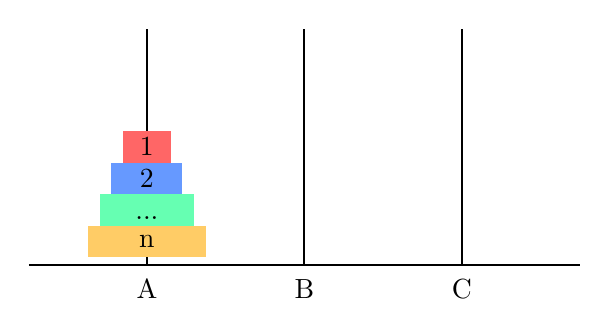
\begin{tikzpicture}

        % 定义圆盘的颜色
        \definecolor{disk1}{RGB}{255, 102, 102}
        \definecolor{disk2}{RGB}{102, 153, 255}
        \definecolor{disk3}{RGB}{102, 255, 178}
        \definecolor{disk4}{RGB}{255, 204, 102}

        % 绘制底座
        \draw[thick] (-2.5, 0) -- (4.5, 0);

        % 绘制三根柱子
        \foreach \x in {-1, 1, 3} {
            \draw[thick] (\x, 0) -- (\x, 3);
        }

        \fill[disk4] (-1.75, 0.1) rectangle (-1.75+1.5, 0.5); % 第4个圆盘
        \node at (-1, 0.3) {n}; % 圆盘4

        \fill[disk3] (-1.6, 0.5) rectangle (-1.6+1.2, 0.9); % 第3个圆盘
        \node at (-1, 0.6) {...}; % 圆盘3

        \fill[disk2] (-1.45, 0.9) rectangle (-1.45+0.9, 1.3); % 第2个圆盘
        \node at (-1, 1.1) {2}; % 圆盘2

        \fill[disk1] (-1.3, 1.3) rectangle (-1.3+0.6, 1.7); % 第1个圆盘
        \node at (-1, 1.5) {1}; % 圆盘1

        % 添加柱子的标签
        \node at (-1, -0.3) {A};
        \node at (1, -0.3) {B};
        \node at (3, -0.3) {C};

    \end{tikzpicture}

\end{frame}
%------------------------------------------------------------

%------------------------------------------------------------
\begin{frame}[fragile]
    \frametitle{例 11.4:汉诺塔问题}
    
    \begin{exampleblock}{编程题}
        \begin{itemize}
            \item 有 A、B、C 这 $3$ 根柱子,A 柱上有 $n (1 \le n \le 20)$ 个圆盘,从上到下给圆盘编号为 $1 \sim n$ ,
                要求按照汉诺塔的移动规则,将 A 柱上的圆盘都移动到 C 柱上。\\
                请输出移动次数最少的移动方案。
        \end{itemize}

        \vspace{1em}

        \begin{columns}

            \column{.01\textwidth}

            \column{.40\textwidth}
            \begin{itemize}
                \item 输入样例\\
                    \lstinline|2|
                \item 输出样例\\
                    \lstinline|Move 1 from A to B|
                    \lstinline|Move 2 from A to C|
                    \lstinline|Move 1 from B to C|
            \end{itemize}

            \column{.60\textwidth}
            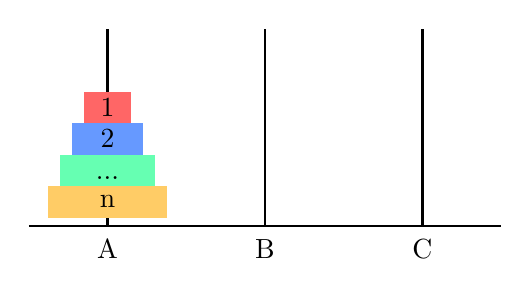
\begin{tikzpicture}

                % 定义圆盘的颜色
                \definecolor{disk1}{RGB}{255, 102, 102}
                \definecolor{disk2}{RGB}{102, 153, 255}
                \definecolor{disk3}{RGB}{102, 255, 178}
                \definecolor{disk4}{RGB}{255, 204, 102}
        
                % 绘制底座
                \draw[thick] (-2, 0) -- (4, 0);
        
                % 绘制三根柱子
                \foreach \x in {-1, 1, 3} {
                    \draw[thick] (\x, 0) -- (\x, 2.5);
                }
        
                \fill[disk4] (-1.75, 0.1) rectangle (-1.75+1.5, 0.5); % 第4个圆盘
                \node at (-1, 0.3) {n}; % 圆盘4
        
                \fill[disk3] (-1.6, 0.5) rectangle (-1.6+1.2, 0.9); % 第3个圆盘
                \node at (-1, 0.6) {...}; % 圆盘3
        
                \fill[disk2] (-1.45, 0.9) rectangle (-1.45+0.9, 1.3); % 第2个圆盘
                \node at (-1, 1.1) {2}; % 圆盘2
        
                \fill[disk1] (-1.3, 1.3) rectangle (-1.3+0.6, 1.7); % 第1个圆盘
                \node at (-1, 1.5) {1}; % 圆盘1
        
                % 添加柱子的标签
                \node at (-1, -0.3) {A};
                \node at (1, -0.3) {B};
                \node at (3, -0.3) {C};
        
            \end{tikzpicture}
        \end{columns}
    \end{exampleblock}

\end{frame}
%------------------------------------------------------------

%------------------------------------------------------------
\begin{frame}[fragile]
    \frametitle{n = 1 的情况}
    
    \begin{itemize}
        \item 直接移动,至少需要 $1$ 次
    \end{itemize}

    \vspace{1em}

    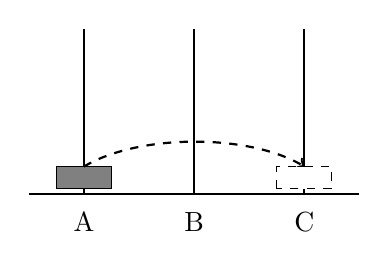
\begin{tikzpicture}[scale=0.7]  % 使用 scale 调整整体大小

        % 绘制底座
        \draw[thick] (0, 0) -- (6, 0);

        % 绘制三根柱子
        \draw[thick] (1,0) -- (1,3); % A柱
        \draw[thick] (3,0) -- (3,3); % B柱
        \draw[thick] (5,0) -- (5,3); % C柱
        
        % 绘制 A 柱上的圆盘
        \filldraw[fill=gray] (0.5,0.1) rectangle (1.5,0.5); % A柱上的圆盘
        
        % 绘制虚线圆弧,箭头指向 C 柱
        \draw[dashed,->,thick] (1,0.5) .. controls (2,1.1) and (4,1.1) .. (5,0.5);
        
        % 在 C 柱上绘制虚线圆盘表示落点
        \filldraw[fill=white, draw=black, dashed] (4.5,0.1) rectangle (5.5,0.5); % C柱上的虚线圆盘
        
        % 标签
        \node at (1,-0.5) {A};
        \node at (3,-0.5) {B};
        \node at (5,-0.5) {C};

    \end{tikzpicture}

\end{frame}
%------------------------------------------------------------

%------------------------------------------------------------
\begin{frame}[fragile]
    \frametitle{n = 2 的情况}
    
    \begin{itemize}
        \only<1> {\item 如何移动可以使得移动次数最少?}
        \item<2-> 把 $2$ 个圆盘 A 柱移动到 C 柱至少需要 $3$ 次移动
        \begin{enumerate}
            \item<3-> 把 A 柱的第 $1$ 个圆盘移动到 B 柱
            \item<4-> 把 A 柱的第 $2$ 个圆盘移动到 C 柱
            \item<5-> 把 B 柱的第 $1$ 个圆盘移动到 C 柱
        \end{enumerate}
        \item<6> 不管把 $2$ 个圆盘从哪个柱移动到另外哪个柱,都至少需要 $3$ 次移动
    \end{itemize}

    \vspace{1em}

    \begin{columns}

    \column{.50\textwidth}
    \only<3-4> {
        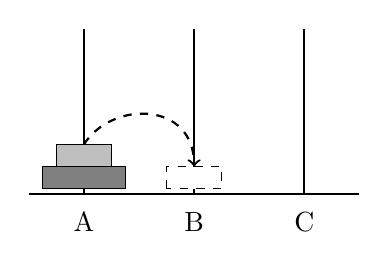
\begin{tikzpicture}[scale=0.7]  % 使用 scale 调整整体大小
        
            % 绘制底座
            \draw[thick] (0, 0) -- (6, 0);
        
            % 绘制三根柱子
            \draw[thick] (1,0) -- (1,3); % A柱
            \draw[thick] (3,0) -- (3,3); % B柱
            \draw[thick] (5,0) -- (5,3); % C柱
            
            % 绘制 A 柱上的两个圆盘
            \filldraw[fill=gray] (0.25,0.1) rectangle (1.75,0.5); % A柱上的第一个圆盘
            \filldraw[fill=lightgray] (0.5,0.5) rectangle (1.5,0.9); % A柱上的第二个圆盘
        
            % 绘制虚线圆弧,箭头指向 B 柱
            \draw[dashed,->,thick] (1,0.9) .. controls (1.5,1.7) and (3,1.7) .. (3,0.5); % 从 A 到 B
        
            % 在 B 柱上绘制虚线圆盘表示落点
            \filldraw[fill=white, draw=black, dashed] (2.5,0.1) rectangle (3.5,0.5); % B柱上的虚线圆盘
        
            % 标签
            \node at (1,-0.5) {A};
            \node at (3,-0.5) {B};
            \node at (5,-0.5) {C};
        
        \end{tikzpicture}
    }
    \only<5-6> {
        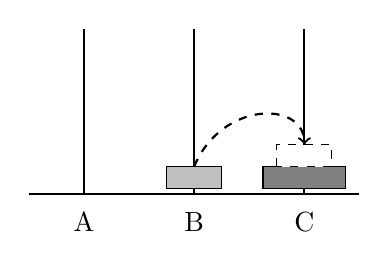
\begin{tikzpicture}[scale=0.7]  % 使用 scale 调整整体大小
        
            % 绘制底座
            \draw[thick] (0, 0) -- (6, 0);
        
            % 绘制三根柱子
            \draw[thick] (1,0) -- (1,3); % A柱
            \draw[thick] (3,0) -- (3,3); % B柱
            \draw[thick] (5,0) -- (5,3); % C柱
            
            % 绘制 A 柱上的两个圆盘
            \filldraw[fill=gray] (4.25,0.1) rectangle (5.75,0.5); % C柱上的第一个圆盘
            \filldraw[fill=lightgray] (2.5,0.1) rectangle (3.5,0.5); % B柱上的第二个圆盘
        
            % 绘制虚线圆弧,箭头指向 C 柱
            \draw[dashed,->,thick] (3,0.5) .. controls (3.5,1.7) and (5,1.7) .. (5,0.9); % 从 A 到 C
        
            % 在 C 柱上绘制虚线圆盘表示落点
            \filldraw[fill=white, draw=black, dashed] (4.5,0.5) rectangle (5.5,0.9); % C柱上的虚线圆盘
        
            % 标签
            \node at (1,-0.5) {A};
            \node at (3,-0.5) {B};
            \node at (5,-0.5) {C};
        
        \end{tikzpicture}
    }

    \column{.50\textwidth}
    \only<4>{
        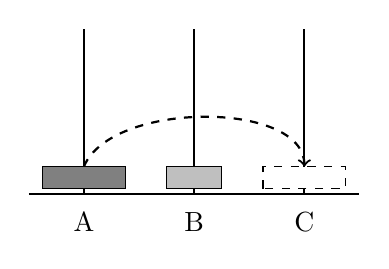
\begin{tikzpicture}[scale=0.7]  % 使用 scale 调整整体大小
        
            % 绘制底座
            \draw[thick] (0, 0) -- (6, 0);
        
            % 绘制三根柱子
            \draw[thick] (1,0) -- (1,3); % A柱
            \draw[thick] (3,0) -- (3,3); % B柱
            \draw[thick] (5,0) -- (5,3); % C柱
            
            % 绘制 A 柱上的两个圆盘
            \filldraw[fill=gray] (0.25,0.1) rectangle (1.75,0.5); % A柱上的第一个圆盘
            \filldraw[fill=lightgray] (2.5,0.1) rectangle (3.5,0.5); % B柱上的第二个圆盘
        
            % 绘制虚线圆弧,箭头指向 B 柱
            \draw[dashed,->,thick] (1,0.5) .. controls (1.5,1.7) and (5,1.7) .. (5,0.5); % 从 A 到 C
        
            % 在 C 柱上绘制虚线圆盘表示落点
            \filldraw[fill=white, draw=black, dashed] (4.25,0.1) rectangle (5.75,0.5); % C柱上的虚线圆盘
        
            % 标签
            \node at (1,-0.5) {A};
            \node at (3,-0.5) {B};
            \node at (5,-0.5) {C};
        
        \end{tikzpicture}
    }
    \only<6> {
        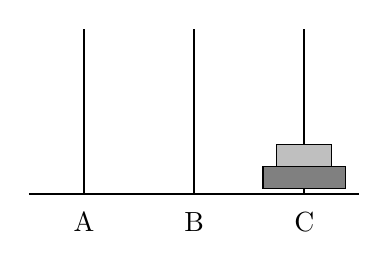
\begin{tikzpicture}[scale=0.7]  % 使用 scale 调整整体大小
        
            % 绘制底座
            \draw[thick] (0, 0) -- (6, 0);
        
            % 绘制三根柱子
            \draw[thick] (1,0) -- (1,3); % A柱
            \draw[thick] (3,0) -- (3,3); % B柱
            \draw[thick] (5,0) -- (5,3); % C柱
            
            % 绘制 A 柱上的两个圆盘
            \filldraw[fill=gray] (4.25,0.1) rectangle (5.75,0.5); % C柱上的第一个圆盘
            \filldraw[fill=lightgray] (4.5,0.5) rectangle (5.5,0.9); % B柱上的第二个圆盘
        
            % 标签
            \node at (1,-0.5) {A};
            \node at (3,-0.5) {B};
            \node at (5,-0.5) {C};
        
        \end{tikzpicture}
    }
    
    \end{columns}

\end{frame}
%------------------------------------------------------------

%------------------------------------------------------------
\begin{frame}[fragile]
    \frametitle{n = 3 的情况}
    
    \begin{itemize}
        \item<2-> 把 A 柱上面的 $2$ 个圆盘在汉诺塔的规则下用最少次数移动(简称“汉诺移”)到 B 柱
        \item<3-> 把 A 柱的第 $3$ 个圆盘移动到 C 柱
        \item<4-> 把 B 柱的 $2$ 个圆盘“汉诺移”到 C 柱
    \end{itemize}

    \vspace{1em}

    \begin{columns}

    \column{.50\textwidth}
    \only<2-3>{
    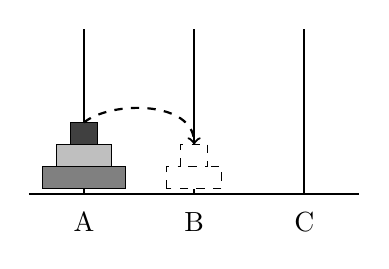
\begin{tikzpicture}[scale=0.7]  % 使用 scale 调整整体大小
    
        % 绘制底座
        \draw[thick] (0, 0) -- (6, 0);
    
        % 绘制三根柱子
        \draw[thick] (1,0) -- (1,3); % A柱
        \draw[thick] (3,0) -- (3,3); % B柱
        \draw[thick] (5,0) -- (5,3); % C柱
        
        % 绘制 A 柱上的三个圆盘
        \filldraw[fill=gray] (0.25,0.1) rectangle (1.75,0.5); % A柱上的第一个圆盘
        \filldraw[fill=lightgray] (0.5,0.5) rectangle (1.5,0.9); % A柱上的第二个圆盘
        \filldraw[fill=darkgray] (0.75,0.9) rectangle (1.25,1.3); % A柱上的第三个圆盘
    
        % 绘制虚线圆弧,箭头指向 B 柱
        \draw[dashed,->,thick] (1,1.3) .. controls (1.5,1.7) and (3,1.7) .. (3,0.9); % 从 A 到 B
    
        % 在 B 柱上绘制虚线圆盘表示落点
        \filldraw[fill=white, draw=black, dashed] (2.5,0.1) rectangle (3.5,0.5); % B柱上的虚线圆盘
        \filldraw[fill=white, draw=black, dashed] (2.75,0.5) rectangle (3.25,0.9); % B柱上的虚线圆盘

        % 标签
        \node at (1,-0.5) {A};
        \node at (3,-0.5) {B};
        \node at (5,-0.5) {C};
    
    \end{tikzpicture}
    }

    \only<4-5>{
    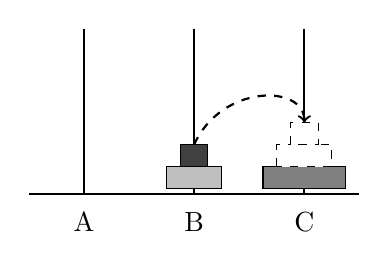
\begin{tikzpicture}[scale=0.7]  % 使用 scale 调整整体大小
    
        % 绘制底座
        \draw[thick] (0, 0) -- (6, 0);
    
        % 绘制三根柱子
        \draw[thick] (1,0) -- (1,3); % A柱
        \draw[thick] (3,0) -- (3,3); % B柱
        \draw[thick] (5,0) -- (5,3); % C柱
        
        % 绘制 A 柱上的两个圆盘
        \filldraw[fill=gray] (4.25,0.1) rectangle (5.75,0.5); % A柱上的第一个圆盘
        \filldraw[fill=lightgray] (2.5,0.1) rectangle (3.5,0.5); % B柱上的第二个圆盘
        \filldraw[fill=darkgray] (2.75,0.5) rectangle (3.25,0.9); % B柱上的第三个圆盘
    
        % 绘制虚线圆弧,箭头指向 C 柱
        \draw[dashed,->,thick] (3,0.9) .. controls (3.5,2) and (5,2) .. (5,1.3); % 从 A 到 C
    
        % 在 C 柱上绘制虚线圆盘表示落点
        \filldraw[fill=white, draw=black, dashed] (4.5,0.5) rectangle (5.5,0.9); % C柱上的虚线圆盘
        \filldraw[fill=white, draw=black, dashed] (4.75,0.9) rectangle (5.25,1.3); % C柱上的虚线圆盘

        % 标签
        \node at (1,-0.5) {A};
        \node at (3,-0.5) {B};
        \node at (5,-0.5) {C};
    
    \end{tikzpicture}
    }

    \column{.50\textwidth}
    \only<3>{
    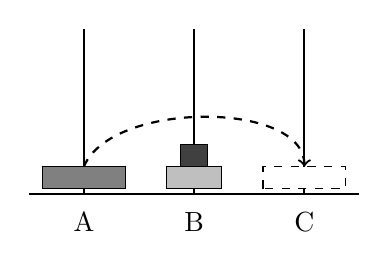
\begin{tikzpicture}[scale=0.7]  % 使用 scale 调整整体大小
        
        % 绘制底座
        \draw[thick] (0, 0) -- (6, 0);
    
        % 绘制三根柱子
        \draw[thick] (1,0) -- (1,3); % A柱
        \draw[thick] (3,0) -- (3,3); % B柱
        \draw[thick] (5,0) -- (5,3); % C柱
            
        % 绘制 A 柱上的两个圆盘
        \filldraw[fill=gray] (0.25,0.1) rectangle (1.75,0.5); % A柱上的第一个圆盘
        \filldraw[fill=lightgray] (2.5,0.1) rectangle (3.5,0.5); % B柱上的第二个圆盘
        \filldraw[fill=darkgray] (2.75,0.5) rectangle (3.25,0.9); % B柱上的第三个圆盘
    
        % 绘制虚线圆弧,箭头指向 C 柱
        \draw[dashed,->,thick] (1,0.5) .. controls (1.5,1.7) and (5,1.7) .. (5,0.5); % 从 A 到 C
    
        % 在 C 柱上绘制虚线圆盘表示落点
        \filldraw[fill=white, draw=black, dashed] (4.25,0.1) rectangle (5.75,0.5); % C柱上的虚线圆盘

        % 标签
        \node at (1,-0.5) {A};
        \node at (3,-0.5) {B};
        \node at (5,-0.5) {C};
    
    \end{tikzpicture}
    }

    \only<5>{
        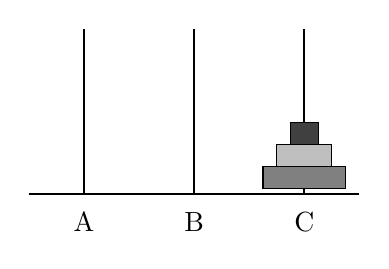
\begin{tikzpicture}[scale=0.7]  % 使用 scale 调整整体大小
            
            % 绘制底座
            \draw[thick] (0, 0) -- (6, 0);
        
            % 绘制三根柱子
            \draw[thick] (1,0) -- (1,3); % A柱
            \draw[thick] (3,0) -- (3,3); % B柱
            \draw[thick] (5,0) -- (5,3); % C柱
                
            % 绘制 A 柱上的两个圆盘
            \filldraw[fill=gray] (4.25,0.1) rectangle (5.75,0.5); % A柱上的第一个圆盘
            \filldraw[fill=lightgray] (4.5,0.5) rectangle (5.5,0.9); % B柱上的第二个圆盘
            \filldraw[fill=darkgray] (4.75,0.9) rectangle (5.25,1.3); % B柱上的第三个圆盘
    
            % 标签
            \node at (1,-0.5) {A};
            \node at (3,-0.5) {B};
            \node at (5,-0.5) {C};
        
        \end{tikzpicture}
        }
    
    \end{columns}

\end{frame}
%------------------------------------------------------------

%------------------------------------------------------------
\begin{frame}[fragile]
    \frametitle{n = x 的情况}
    
    \begin{itemize}
        \item<2-> 把 A 柱上面的 $x - 1$ 个圆盘“汉诺移”到 B 柱
        \item<3-> 把 A 柱的第 $x$ 个圆盘移动到 C 柱
        \item<4-> 把 B 柱的 $x - 1$ 个圆盘“汉诺移”到 C 柱
        \item<5-> 重复的操作:“汉诺移”
        \item<6-> 子问题:将 $x - 1$ 个圆盘从某个柱“汉诺移”到另一个柱的方案
    \end{itemize}

    \vspace{1em}

    \begin{columns}

    \column{.50\textwidth}
    \only<2-3>{
    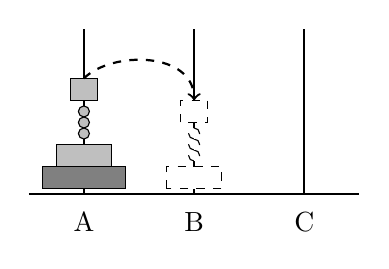
\begin{tikzpicture}[scale=0.7]  % 使用 scale 调整整体大小
    
        % 绘制底座
        \draw[thick] (0, 0) -- (6, 0);
    
        % 绘制三根柱子
        \draw[thick] (1,0) -- (1,3); % A柱
        \draw[thick] (3,0) -- (3,3); % B柱
        \draw[thick] (5,0) -- (5,3); % C柱
        
        % 绘制 A 柱上的三个圆盘
        \filldraw[fill=gray] (0.25,0.1) rectangle (1.75,0.5); % A柱上的第一个圆盘
        \filldraw[fill=lightgray] (0.5,0.5) rectangle (1.5,0.9); % A柱上的第二个圆盘
        \filldraw[fill=lightgray] (0.75,1.7) rectangle (1.25,2.1); % A柱上的第三个圆盘
        \filldraw[fill=lightgray] (1,1.1) circle (0.1);  % 绘制一个圆点
        \filldraw[fill=lightgray] (1,1.3) circle (0.1);  % 绘制一个圆点
        \filldraw[fill=lightgray] (1,1.5) circle (0.1);  % 绘制一个圆点
    
        % 绘制虚线圆弧,箭头指向 B 柱
        \draw[dashed,->,thick] (1,2.1) .. controls (1.5,2.6) and (3,2.6) .. (3,1.7); % 从 A 到 B
    
        % 在 B 柱上绘制虚线圆盘表示落点
        \filldraw[fill=white, draw=black, dashed] (2.5,0.1) rectangle (3.5,0.5); % B柱上的虚线圆盘
        \filldraw[fill=white, draw=black, dashed] (2.75,1.7-0.4) rectangle (3.25,2.1-0.4); % B柱上的虚线圆盘
        \filldraw[fill=white, draw=black, dashed] (3,1.1-0.4) circle (0.1);  % 绘制一个圆点
        \filldraw[fill=white, draw=black, dashed] (3,1.3-0.4) circle (0.1);  % 绘制一个圆点
        \filldraw[fill=white, draw=black, dashed] (3,1.5-0.4) circle (0.1);  % 绘制一个圆点

        % 标签
        \node at (1,-0.5) {A};
        \node at (3,-0.5) {B};
        \node at (5,-0.5) {C};
    
    \end{tikzpicture}
    }

    \only<4->{
    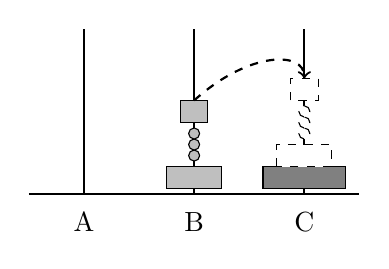
\begin{tikzpicture}[scale=0.7]  % 使用 scale 调整整体大小
    
        % 绘制底座
        \draw[thick] (0, 0) -- (6, 0);
    
        % 绘制三根柱子
        \draw[thick] (1,0) -- (1,3); % A柱
        \draw[thick] (3,0) -- (3,3); % B柱
        \draw[thick] (5,0) -- (5,3); % C柱
        
        % 绘制 A 柱上的三个圆盘
        \filldraw[fill=gray] (4.25,0.1) rectangle (5.75,0.5); % A柱上的第一个圆盘
        \filldraw[fill=lightgray] (2.5,0.1) rectangle (3.5,0.5); % B柱上的虚线圆盘
        \filldraw[fill=lightgray] (2.75,1.7-0.4) rectangle (3.25,2.1-0.4); % B柱上的虚线圆盘
        \filldraw[fill=lightgray] (3,1.1-0.4) circle (0.1);  % 绘制一个圆点
        \filldraw[fill=lightgray] (3,1.3-0.4) circle (0.1);  % 绘制一个圆点
        \filldraw[fill=lightgray] (3,1.5-0.4) circle (0.1);  % 绘制一个圆点
    
        % 绘制虚线圆弧,箭头指向 B 柱
        \draw[dashed,->,thick] (3,1.7) .. controls (4,2.6) and (5,2.6) .. (5,2.1); % 从 A 到 B
    
        % 在 B 柱上绘制虚线圆盘表示落点
        \filldraw[fill=white, draw=black, dashed] (4.5,0.5) rectangle (5.5,0.9); % B柱上的虚线圆盘
        \filldraw[fill=white, draw=black, dashed] (4.75,1.7) rectangle (5.25,2.1); % B柱上的虚线圆盘
        \filldraw[fill=white, draw=black, dashed] (5,1.1) circle (0.1);  % 绘制一个圆点
        \filldraw[fill=white, draw=black, dashed] (5,1.3) circle (0.1);  % 绘制一个圆点
        \filldraw[fill=white, draw=black, dashed] (5,1.5) circle (0.1);  % 绘制一个圆点
        % 标签
        \node at (1,-0.5) {A};
        \node at (3,-0.5) {B};
        \node at (5,-0.5) {C};
    
    \end{tikzpicture}
    }

    \column{.50\textwidth}
    \only<3>{
    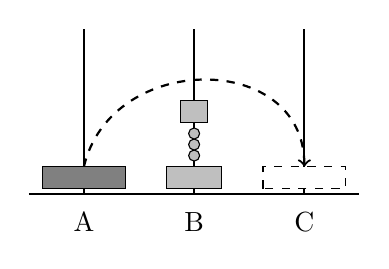
\begin{tikzpicture}[scale=0.7]  % 使用 scale 调整整体大小
        
        % 绘制底座
        \draw[thick] (0, 0) -- (6, 0);
    
        % 绘制三根柱子
        \draw[thick] (1,0) -- (1,3); % A柱
        \draw[thick] (3,0) -- (3,3); % B柱
        \draw[thick] (5,0) -- (5,3); % C柱
            
        % 绘制 A 柱上的三个圆盘
        \filldraw[fill=gray] (0.25,0.1) rectangle (1.75,0.5); % A柱上的第一个圆盘
        \filldraw[fill=lightgray] (2.5,0.1) rectangle (3.5,0.5); % B柱上的虚线圆盘
        \filldraw[fill=lightgray] (2.75,1.7-0.4) rectangle (3.25,2.1-0.4); % B柱上的虚线圆盘
        \filldraw[fill=lightgray] (3,1.1-0.4) circle (0.1);  % 绘制一个圆点
        \filldraw[fill=lightgray] (3,1.3-0.4) circle (0.1);  % 绘制一个圆点
        \filldraw[fill=lightgray] (3,1.5-0.4) circle (0.1);  % 绘制一个圆点
    
        % 绘制虚线圆弧,箭头指向 B 柱
        \draw[dashed,->,thick] (1,0.5) .. controls (1.5,2.6) and (5,2.6) .. (5,0.5); % 从 A 到 B
    
        % 在 B 柱上绘制虚线圆盘表示落点
        \filldraw[fill=white, draw=black, dashed] (4.25,0.1) rectangle (5.75,0.5); % C柱上的虚线圆盘

        % 标签
        \node at (1,-0.5) {A};
        \node at (3,-0.5) {B};
        \node at (5,-0.5) {C};
    
    \end{tikzpicture}
    }

    \only<5->{
        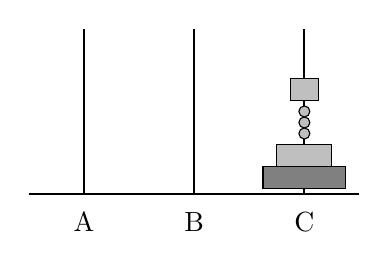
\begin{tikzpicture}[scale=0.7]  % 使用 scale 调整整体大小
            
            % 绘制底座
            \draw[thick] (0, 0) -- (6, 0);
        
            % 绘制三根柱子
            \draw[thick] (1,0) -- (1,3); % A柱
            \draw[thick] (3,0) -- (3,3); % B柱
            \draw[thick] (5,0) -- (5,3); % C柱
                
            % 绘制 A 柱上的三个圆盘
            \filldraw[fill=gray] (4.25,0.1) rectangle (5.75,0.5); % A柱上的第一个圆盘
            \filldraw[fill=lightgray] (4.5,0.5) rectangle (5.5,0.9); % B柱上的虚线圆盘
            \filldraw[fill=lightgray] (4.75,1.7) rectangle (5.25,2.1); % B柱上的虚线圆盘
            \filldraw[fill=lightgray] (5,1.1) circle (0.1);  % 绘制一个圆点
            \filldraw[fill=lightgray] (5,1.3) circle (0.1);  % 绘制一个圆点
            \filldraw[fill=lightgray] (5,1.5) circle (0.1);  % 绘制一个圆点
    
            % 标签
            \node at (1,-0.5) {A};
            \node at (3,-0.5) {B};
            \node at (5,-0.5) {C};
        
        \end{tikzpicture}
        }
    
    \end{columns}

\end{frame}
%------------------------------------------------------------

%------------------------------------------------------------
\begin{frame}[fragile]
    \frametitle{函数思路}
    
    \begin{itemize}
        \item 定义函数 \lstinline|hanoiMove(x, start, target, other)| 的功能是输出 $x$ 个圆盘(编号 $1 \sim x$ )从 start 柱“汉诺移”到 target 柱的移动方案
        \begin{itemize}
            \item 输出 start 柱编号 $1 \sim x - 1$ 的圆盘“汉诺移”到 other 柱的方案,调用 \lstinline|hanoiMove(x - 1, start, other, target)|
            \item 将 start 柱编号 $x$ 的圆盘移动到 target 柱,直接输出
            \item 输出 other 柱编号 $1 \sim x - 1$ 的圆盘“汉诺移”到 target 柱的方案,调用 \lstinline|hanoiMove(x - 1, other, target, start)|
        \end{itemize}
        \item 最简子问题:\lstinline|x == 1| 时直接移动,或 \lstinline|x == 0| 时不用移动
    \end{itemize}

\end{frame}
%------------------------------------------------------------

%------------------------------------------------------------
\begin{frame}[fragile]
    \frametitle{代码示例}
    
    \lstinputlisting[basicstyle=\ttfamily\footnotesize,language=C++,name=hanoi]{ch23/hanoi.cc}

\end{frame}
%------------------------------------------------------------

%------------------------------------------------------------
\begin{frame}[fragile]
    \frametitle{函数思路}
    
    \begin{tikzpicture}[node distance=1cm and 1cm, % 控制节点之间的距离
        every node/.style={rectangle, draw, rounded corners, align=center, minimum width=0.4cm, minimum height=0.5cm}  % 设置节点样式
    ]
    
    % 定义节点
    \node (n1) {\lstinline|hanoiMove|\\\lstinline|(3,A,C,B)|};
    \node (n2) [below left=of n1] {\lstinline|hanoiMove|\\\lstinline|(2,A,B,C)|\\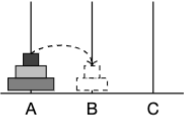
\includegraphics[width=2cm]{ch23/p00}};
    \node (n3) [below =of n2] {\lstinline|Move 2|\\\lstinline|A->B|};
    \node (n4) [left=0.2cm of n3] {\lstinline|hanoiMove|\\\lstinline|(1,A,C,B)|};
    \node (n5) [right=0.2cm of n3] {\lstinline|hanoiMove|\\\lstinline|(1,C,B,A)|};
    \node (n6) [below =of n1] {\lstinline|Move 3 A->B|\\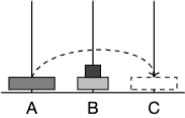
\includegraphics[width=2cm]{ch23/p01}};
    \node (n7) [below right=of n1] {\lstinline|hanoiMove|\\\lstinline|(2,C,A,B)|\\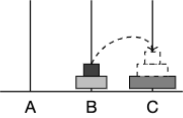
\includegraphics[width=2cm]{ch23/p02}};
    \node (n71) [below = of n7] {\lstinline|...|};
    \node (n72) [left=0.2cm of n71] {\lstinline|...|};
    \node (n73) [right=0.2cm of n71] {\lstinline|...|};
    
    % 绘制连线
    \draw[->] (n1.south) -- (n2.north);
    \draw[->] (n1.south) -- (n6.north);
    \draw[->] (n1.south) -- (n7.north);

    \draw[->] (n2.south) -- (n3.north);
    \draw[->] (n2.south) -- (n4.north);
    \draw[->] (n2.south) -- (n5.north);
    
    \draw[->] (n7.south) -- (n71.north);
    \draw[->] (n7.south) -- (n72.north);
    \draw[->] (n7.south) -- (n73.north);
   
    \end{tikzpicture}
    

\end{frame}
%------------------------------------------------------------

%------------------------------------------------------------
\begin{frame}[fragile]
    \frametitle{函数思路}
    
    \begin{exampleblock}{编程题}
        \begin{itemize}
            \item 有 A、B、C 这 $3$ 根柱子,A 柱上有 $n (1 \le n \le 20)$ 个圆盘,从上到下给圆盘编号为 $1 \sim n$ ,
                要求按照汉诺塔的移动规则,将 A 柱上的圆盘都移动到 C 柱上。\\
                求其最少的移动次数。
        \end{itemize}
    
        \vspace{1em}
    
        \begin{columns}
    
            \column{.01\textwidth}
    
            \column{.40\textwidth}
            \begin{itemize}
                \item 输入样例\\
                    \lstinline|2|
                \item 输出样例\\
                    \lstinline|3|
            \end{itemize}
    
            \column{.60\textwidth}
            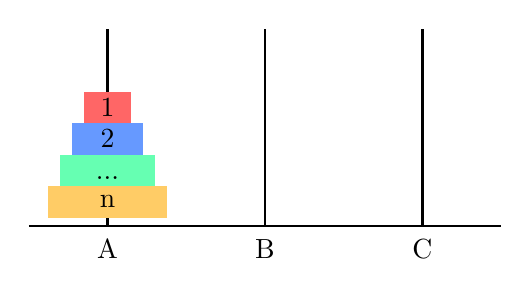
\begin{tikzpicture}
    
                % 定义圆盘的颜色
                \definecolor{disk1}{RGB}{255, 102, 102}
                \definecolor{disk2}{RGB}{102, 153, 255}
                \definecolor{disk3}{RGB}{102, 255, 178}
                \definecolor{disk4}{RGB}{255, 204, 102}
        
                % 绘制底座
                \draw[thick] (-2, 0) -- (4, 0);
        
                % 绘制三根柱子
                \foreach \x in {-1, 1, 3} {
                    \draw[thick] (\x, 0) -- (\x, 2.5);
                }
        
                \fill[disk4] (-1.75, 0.1) rectangle (-1.75+1.5, 0.5); % 第4个圆盘
                \node at (-1, 0.3) {n}; % 圆盘4
        
                \fill[disk3] (-1.6, 0.5) rectangle (-1.6+1.2, 0.9); % 第3个圆盘
                \node at (-1, 0.6) {...}; % 圆盘3
        
                \fill[disk2] (-1.45, 0.9) rectangle (-1.45+0.9, 1.3); % 第2个圆盘
                \node at (-1, 1.1) {2}; % 圆盘2
        
                \fill[disk1] (-1.3, 1.3) rectangle (-1.3+0.6, 1.7); % 第1个圆盘
                \node at (-1, 1.5) {1}; % 圆盘1
        
                % 添加柱子的标签
                \node at (-1, -0.3) {A};
                \node at (1, -0.3) {B};
                \node at (3, -0.3) {C};
        
            \end{tikzpicture}
        \end{columns}
    \end{exampleblock}

\end{frame}
%------------------------------------------------------------

%------------------------------------------------------------
\begin{frame}[fragile]
    \frametitle{函数思路}
    
    \begin{itemize}
        \item 定义函数 \lstinline|hanoiCnt(x, start, target, other)| 的功能是计算 $x$ 个圆盘从 start 柱“汉诺移”到 target 柱需要移动的次数
        \begin{itemize}
            \item $x$ 表示圆盘个数,\lstinline|int| 类型
            \item \lstinline|start, target, other| 表示柱子,为 \lstinline|'A', 'B', 'C'| 之一,\lstinline|char| 类型
            \item 返回值表示移动次数,\lstinline|int| 类型
        \end{itemize}
    \end{itemize}

\end{frame}
%------------------------------------------------------------

%------------------------------------------------------------
\begin{frame}[fragile]
    \frametitle{递归函数分析}
    
    \begin{itemize}
        \item \lstinline|hanoiCnt(x, start, target, other)| 的实现
        \begin{itemize}
            \item 把 start 柱上面的 $x - 1$ 个圆盘“汉诺移”到 other 柱,需要 \lstinline|hanoiCnt(x - 1, start, other, target)| 次
            \item 把 start 柱第 $x$ 个圆盘移动到 target 柱,需要 $1$ 次
            \item 把 other 柱的 $x - 1$ 个圆盘“汉诺移”到 target 柱,需要 \lstinline|hanoiCnt(x - 1, other, target, start)| 次
            \item 最简子问题:\lstinline|x == 1| 时,移动 $1$ 次
        \end{itemize}
    \end{itemize}

\end{frame}
%------------------------------------------------------------

%------------------------------------------------------------
\begin{frame}[fragile]
    \frametitle{代码示例}
    
    \only<1>{\lstinputlisting[basicstyle=\ttfamily\footnotesize,language=C++,name=hanoi_cnt]{ch23/hanoi_cnt.cc}}
    \only<2-4>{
        \lstinputlisting[basicstyle=\ttfamily\footnotesize,language=C++,name=hanoi_cnt2]{ch23/hanoi_cnt2.cc}
        \begin{tikzpicture}[remember picture, overlay]
            \uncover<3->{\redbox{hanoi_cnt2}{2}{24}{2}{50} node[below,yshift=-.5cm]{能不能不要这 3 个参数};}
            \uncover<4>{\redbox{hanoi_cnt2}{2}{24}{2}{50} node[below,yshift=-4cm]{不参与实际运算,可以不要};}
        \end{tikzpicture}
    }

    \only<5-7> {
        \begin{columns}
            \column{.50\textwidth}
            \lstinputlisting[basicstyle=\ttfamily\footnotesize,language=C++,name=hanoi_cnt3]{ch23/hanoi_cnt3.cc}
            \begin{tikzpicture}[remember picture, overlay]
                \uncover<6->{\redbox{hanoi_cnt3}{5}{11}{5}{27};}
                \uncover<6->{\redbox{hanoi_cnt3}{7}{11}{7}{27};}
            \end{tikzpicture}

            \column{.50\textwidth}
            \uncover<7>{\lstinputlisting[basicstyle=\ttfamily\footnotesize,language=C++,name=hanoi_cnt4]{ch23/hanoi_cnt4.cc}}
        \end{columns}
    }

\end{frame}
%------------------------------------------------------------


\section{总结}

%------------------------------------------------------------
\begin{frame}[fragile]
    \frametitle{总结}
    
    \begin{itemize}
        \item 递归分析问题的一种方式:
        \begin{itemize}
            \item 根据重复的操作或功能,明确子问题,给递归函数下定义
            \begin{itemize}
                \item 函数的功能要明确
                \item 函数中各个参数的含义与其位置要对应
                \item 函数的返回值及其含义要明确
            \end{itemize}
            \item 在操作需要重复的地方 或 需要达到相同功能的地方,调用函数自身
            \item 根据递归函数的定义,确定最简子问题的答案
        \end{itemize}
        \item 数的精致度、分裂问题、汉诺塔问题
    \end{itemize}

\end{frame}
%------------------------------------------------------------

\end{document}